\subsection{Backpropagation for a simple network}

\subsubsection{Formula for Backpropagation}
\begin{math}
 \delta
\end{math}


Da man mit zufälligen Anfangsgewichten arbeitet kann es vorkommen das man auch unterschiedliche lokale Minima findet.
Dies ist sehr stark von den Werten der Anfangsgewichte abhängig. Bei ``schlechten Startgewichten'' kann es vorkommen das man in ein Lokales Minima läuft.

\begin{figure}[hp!]
\begin{center}
 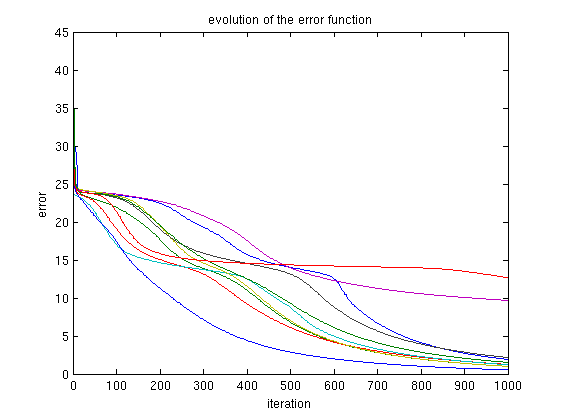
\includegraphics[width=0.99\textwidth]{./figures/1/error}
 \caption{Evolution of the error over the iterations with different startweight-vectors}
\label{fig:backprop_error}
\end{center}
\end{figure}



\begin{figure}[hp!]
\begin{center}
 \begin{minipage}{0.48\textwidth}
 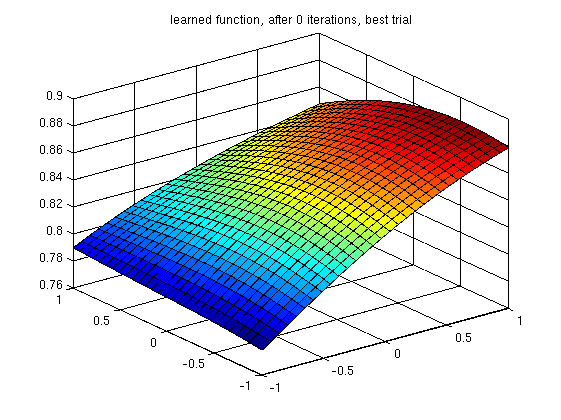
\includegraphics[width=0.99\textwidth]{./figures/1/learned_best_0}
 \end{minipage}
 \begin{minipage}{0.48\textwidth}
 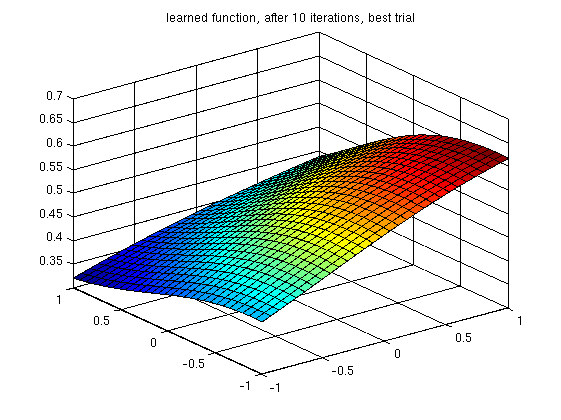
\includegraphics[width=0.99\textwidth]{./figures/1/learned_best_10}
 \end{minipage}
 \begin{minipage}{0.48\textwidth}
 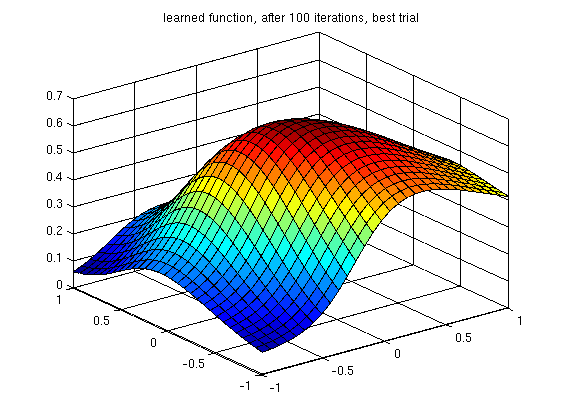
\includegraphics[width=0.99\textwidth]{./figures/1/learned_best_100}
 \end{minipage}
 \begin{minipage}{0.48\textwidth}
 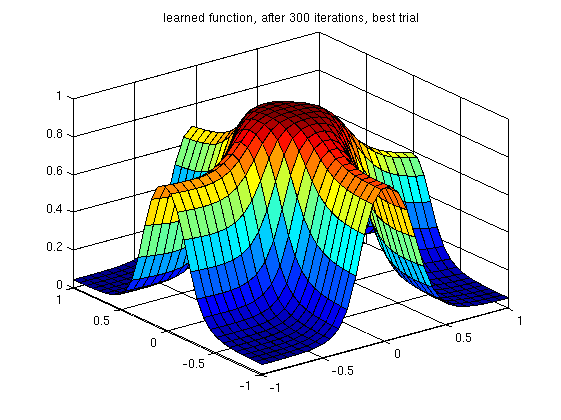
\includegraphics[width=0.99\textwidth]{./figures/1/learned_best_300}
 \end{minipage}
 \begin{minipage}{0.48\textwidth}
 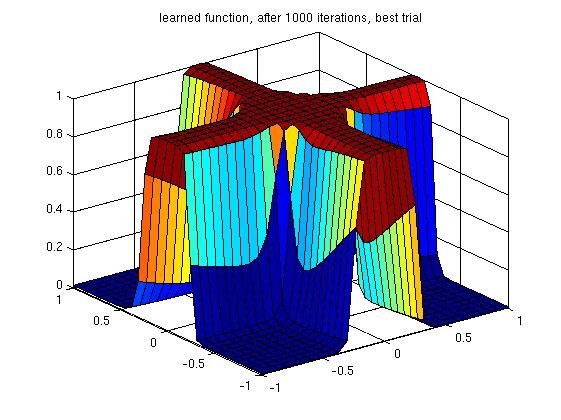
\includegraphics[width=0.99\textwidth]{./figures/1/learned_best_1000}
 \end{minipage}
 \caption{Learned Function after 0,10,100,300,1000 Iterations(Best Trial)}
\label{fig:learned_function_best}
\end{center}
\end{figure}


\begin{figure}[hp!]
\begin{center}
 \begin{minipage}{0.48\textwidth}
 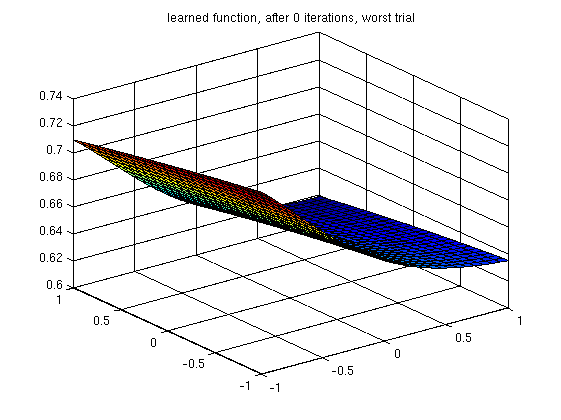
\includegraphics[width=0.99\textwidth]{./figures/1/learned_worst_0}
 \end{minipage}
 \begin{minipage}{0.48\textwidth}
 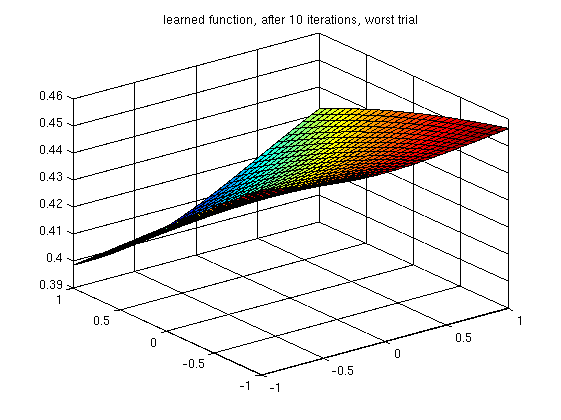
\includegraphics[width=0.99\textwidth]{./figures/1/learned_worst_10}
 \end{minipage}
 \begin{minipage}{0.48\textwidth}
 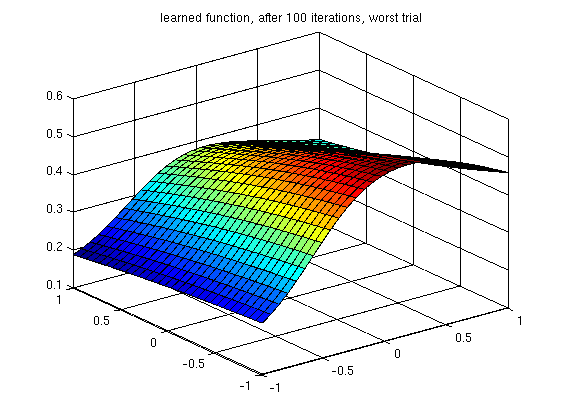
\includegraphics[width=0.99\textwidth]{./figures/1/learned_worst_100}
 \end{minipage}
 \begin{minipage}{0.48\textwidth}
 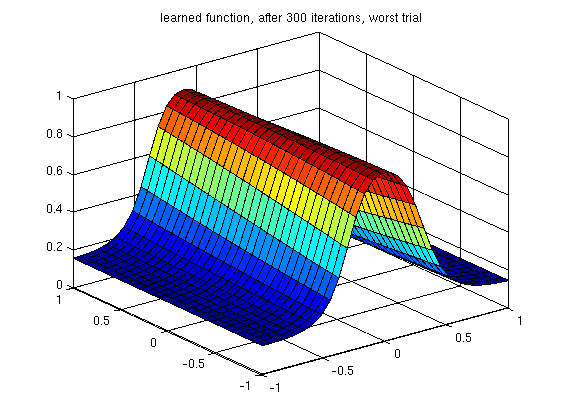
\includegraphics[width=0.99\textwidth]{./figures/1/learned_worst_300}
 \end{minipage}
 \begin{minipage}{0.48\textwidth}
 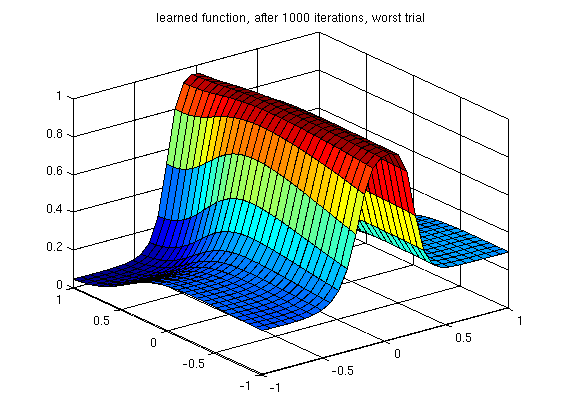
\includegraphics[width=0.99\textwidth]{./figures/1/learned_worst_1000}
 \end{minipage}
 \caption{Learned Function after 0,10,100,300,1000 Iterations(Worst Trial)}
\label{fig:learned_function_worst}
\end{center}
\end{figure}

